\documentclass[12pt,a4paper]{article}
\usepackage[utf8]{inputenc}
\usepackage{amsmath}
\usepackage{amsfonts}
\usepackage{amssymb}
\usepackage{graphicx}
\usepackage{float}
\usepackage[ngerman]{babel}
\parindent0pt


\title{Pflichtenheft E-Learning System}
\author{Matthias Englert, Fabian Schilha, Andreas Rottach}
\date{Wintersemester 2014/2015}

\begin{document}
\maketitle
\newpage
\tableofcontents
\newpage
\section{Überblick}
\subsection{Einleitung}
Dieses Software-Projekt hat sich als Ziel gesetzt eine webbasierte, zentrale E-Learning Plattform für die Studenten der Universität Ulm bereitzustellen. Das System soll die Lerninhalte individuell für jeden Benutzer in geeigneter Form strukturieren. Des Weiteren kann jeder Anwender den Lernstoff erweitern und mit anderen Benutzern darüber diskutieren. Die Lerninhalte werden in einer hierarchischen Struktur mit verschiedenen Detailebenen dargestellt, um unterschiedliche Einblicke in ein Themengebiet zu ermöglichen. Das Skript soll durch verschiedene digitale Inhalte wie Bilder, Texte oder Videos unterstützt werden. Dozenten können initiale Lehrinhalte bereitstellen, die sich im Laufe des Semesters verändern oder erweitern werden können.

\subsection{Motivation}
Zurzeit verfügt die Universität Ulm über viele Plattformen (Moodle, ILIAS, Rubikon und slc) um Vorlesungsmaterialien den Studenten bereitzustellen. Diese Plattformen sind keine echten E-Learning Systeme, da man sie nur nutzt um Dokumente wie Skripte oder Übungsblätter herunterzuladen. Außerdem gibt es als einzige Informationsquelle zum Lernen nur das Skript und keine anderen Medien wie z.B. Videos. Das Skript kann dabei nur in einer festen linearen Struktur durchgearbeitet werden. Lernen ist allerdings kein linearer Prozess, sondern ein Prozess, bei dem Informationen zu einem Netzwerk zusammengebaut werden. Dieses Netzwerk zu erweitern und immer wieder umzustrukturieren stellt den eigentlichen Lernprozess da. Bei einem linearen Skript fehlen dabei Querverweise zu anderen Quellen, falls man einen Begriff beispielsweise nicht versteht. Zu diesem Lernprozess gehört auch, dass man sich mit anderen Studenten austauscht. In den bereits vorhandenen Vorlesungsplattformen lädt jedoch jeder das Skript runter und lernt für sich allein. Es gibt keine Möglichkeit persönliche Notizen im Skript mit anderen zu teilen. Dadurch bekommt auch der Dozent keine Vorstellung davon was man im Skript besser machen könnte, sodass sich das Skript über die Jahre kaum ändert.
Mit unserem E-Learning System wollen wir diese Probleme anpacken! 

\newpage

\subsection{Vision und Leitbild}
Das Ziel des Projekts ist es den Studenten für jede Vorlesung eine zentrale webbasierte Lernumgebung anzubieten. Der Dozent einer Vorlesung hat die Möglichkeit eine Veranstaltung anzulegen, auf der er dann ein initiales Skript bereitstellen kann. Durch die während des Semesters aufkommenden Diskussionen ist er in der Lage das Skript mit Hilfe der Studenten zu erweitern. Die Vorlesungsinhalte sollen dabei nicht mehr linear aufgebaut sein, sondern einzelne Teile (z.B. eine Definition oder ein Satz in der Mathematik) sollen auf Karteikarten gespeichert werden. Die Karteikarten sind hierarchisch angeordnet und zusätzlich durch Querverweise miteinander verknüpft werden, sodass ein Netzwerk entsteht. Dadurch ist es für die Anzeige beispielsweise möglich auf Vorlesungsfolien weniger Information zu packen, als ins Skript, sodass die Anzeige flexibel wird. Durch die Struktur als Netzwerk ist es für einen Student, der beispielsweise ein Matheskript liest und über den Begriff der Differenzialgleichung stößt, möglich zuerst eine kurze Definition zu dem Begriff zu erhalten. Falls dies nicht ausreichend ist, hat er die Wahl sich zwischen verschiedenen Quellen zu diesem Thema zu entscheiden. Beispielsweise könnte er auf ein YouTube-Video oder eine andere Website verlinkt werden. In dem Netzwerk ist es aber trotzdem noch wichtig dass es einen linearen Pfad gibt, der das Skript repräsentiert. Des weiteren soll ein Student zu jeder Karteikarte Notizen machen oder eine Diskussion anstoßen können. Der Student kann entscheiden, ob andere seine Notizen sehen dürfen. Um die Qualität der Diskussion beurteilen zu können, gibt es die Möglichkeit, einzelne Beiträge durch positive Bewertungen hervorzuheben. Außerdem existieren Moderatoren, die die Aufgabe haben, schlechte Beiträge zu entfernen und besonders gute Beiträge ins Skript einzuarbeiten. Die Rolle des Moderators kann z.B. der Dozent oder der Übungsleiter übernehmen.


\section{Projektkontext}
Das Software-System wird im Rahmen des Softwaregrundprojekts Wintersemester 2014/2015 im Bereich Informatik entstehen. Dies kann eventuell in den bestehenden Lehrbetrieb der Universität Ulm eingebettet werden, so dass allen Studenten an der Universität die Möglichkeit zu diesem System angeboten werden kann.

\section{Anforderungsanalyse}
\subsection{Fachwissen (Glossar)}
\begin{tabular}{l p{10cm}}  
BEGRIFF 	 & \textbf{Administrator} \\ 
BESCHREIBUNG & Benutzer mit erweiterten Zugansrechten zur Systemverwaltung\\ 
ISTEIN   	 & Benutzer \\
KANNSEIN 	 & Student, Tutor, Dozent \\ 
ASPEKT   	 & verwaltet die Benutzer und deren Zugangsrechte\\
BEISPIEL 	 & Anreas Rottach(Administrator)\\\\
\hline
\end{tabular}\\\\  

\begin{tabular}{l p{10cm}}
BEGRIFF 	 & \textbf{Benutzer} \\ 
BESCHREIBUNG & Eine Nutzer des E-Learning System \\ 
ISTEIN   	 & Student, Übungsleiter, Dozent, Tutor, Administrator \\
KANNSEIN 	 &   - \\ 
ASPEKT   	 & nutzt das System mit seinen Funktionalitäten\\
BEISPIEL 	 & Heinz Kuntz(Tutor), Ralf Morgen(Student), Nico Walz(Üungsleiter)\\\\
\hline
\end{tabular}\\\\    

\begin{tabular}{l p{10cm}}
BEGRIFF 	 & \textbf{Dozent} \\ 
BESCHREIBUNG & Person die Vorlesungen veranstaltet und abhält \\ 
ISTEIN   	 & Benutzer\\
KANNSEIN 	 & Tutor, Administrator \\ 
ASPEKT   	 & stellt das initiale Skript zur Verfügung, und\\
			 &  hält Vorlesungen in einer Veranstaltung ab\\
BEISPIEL 	 & Prof. Dr. Helmuth Partsch\\\\
\hline
\end{tabular}\\\\   

\begin{tabular}{l p{10cm}}
BEGRIFF 	 & \textbf{eMail-Server} \\ 
BESCHREIBUNG & Datenstruktur zum Nachrichtenversand \\
ISTEIN   	 & System \\
KANNSEIN 	 & - \\ 
ASPEKT   	 & Sicherung und Versand der einzelnen Nachrichten\\
			 & zwischen den Benutzern \\
BEISPIEL 	 & \\\\
\hline
\end{tabular}\\\\   

\begin{tabular}{l p{10cm}}
\hline\\
BEGRIFF 	 & \textbf{Moderator} \\ 
BESCHREIBUNG & Person die Foren überwacht\\
ISTEIN   	 & Benutzer \\
KANNSEIN 	 & Administrator, Tutor, Student \\ 
ASPEKT   	 & überwacht die Diskussionen im System \\
 	     	 & und filtert weiter gute Lehrinhalte und\\
 	     	 & Verbesserungsvorschläge heraus\\
BEISPIEL 	 & Alexander Nasaal\\\\
\hline
\end{tabular}\\\\   

\begin{tabular}{l p{10cm}}
BEGRIFF 	 & \textbf{Student} \\ 
BESCHREIBUNG & Immatrikulierte Person an einer Universität \\ 
ISTEIN   	 & Benutzer \\
KANNSEIN 	 & Anwender, Administrator \\ 
ASPEKT   	 & erweitert die Informationen des Systems\\
 	     	 & und stellt diese anderen Benutzern zur Verfügung \\
BEISPIEL 	 & Mia Zu(Student)\\\\
\hline
\end{tabular}\\\\  

\begin{tabular}{l p{10cm}}
BEGRIFF 	 & \textbf{Person} \\ 
BESCHREIBUNG & ein menschliches Wesen\\ 
ISTEIN   	 & Benutzer\\
KANNSEIN 	 & Student, Administrator, Anwender, Moderator,\\
			 & Dozent, Tutor, Übungsleiter, Benutzer \\ 
ASPEKT   	 & gleichbedeutend wie der Benutzer \\
BEISPIEL 	 & Harald Meier(Person)\\\\
\hline
\end{tabular}\\\\  

\begin{tabular}{l p{10cm}}
BEGRIFF 	 & \textbf{Tutor} \\ 
BESCHREIBUNG & Eine Person an der Universität die den Übungsbetrieb unterstützt\\ 
ISTEIN   	 & Benutzer\\
KANNSEIN 	 & Übungsleiter, Moderator, Student,Administrator\\ 
ASPEKT   	 & unterstützt die Studenten bei Fragen zu Lehrinhalten\\
BEISPIEL 	 & Manuel Güntzel(Tutor)\\\\
\hline
\end{tabular}\\\\  

\begin{tabular}{l p{10cm}}
\hline
BEGRIFF 	 & \textbf{Übungsleiter} \\ 
BESCHREIBUNG & Eine Person an der Universität \\ 
ISTEIN   	 & Tutor\\
KANNSEIN 	 & Moderator, Student, Administrator, Dozent \\ 
ASPEKT   	 & erstellt Übungsblätter und Aufgaben für Studenten \\
BEISPIEL 	 & Alexander Nasaal(Übungsleiter)\\\\
\hline
\end{tabular}\\\\  

\begin{tabular}{l p{10cm}}
BEGRIFF 	 & \textbf{Beiträge} \\ 
BESCHREIBUNG & eine ideelle , oder fachliche Leistung von Benutzern des Systems \\ 
ISTEIN   	 &  -\\
KANNSEIN 	 & Notiz, Daten, Kommentar, Information, Karteikarte, Verbesserungsvorschlag\\ 
ASPEKT   	 & soll den Lernstoff des Systems erweitern und ausbauen\\
BEISPIEL 	 & Manfred Oberhuber stellt ein Notiz für das System zur Verfügung
			 (Ein Beitrag von Manfred Oberhuber )\\\\
\hline
\end{tabular}\\\\  

\begin{tabular}{l p{10cm}}
BEGRIFF 	 & \textbf{Bewertungssystem} \\ 
BESCHREIBUNG & System nach dem eine Bewertung folgt\\ 
ISTEIN   	 & System\\
KANNSEIN 	 & - \\ 
ASPEKT   	 & Studenten können einzelne Beiträge im System bewerten\\
BEISPIEL 	 & Student Oberhuber bewertet eine Karteikarte positiv \\\\
\hline
\end{tabular}\\\\  

\begin{tabular}{l p{10cm}}
BEGRIFF 	 & \textbf{Daten} \\ 
BESCHREIBUNG & Angaben, Beobachtungen, Informationen von Benutzern\\ 
ISTEIN   	 & -\\
KANNSEIN 	 & Notiz, Daten, Kommentar, Information, Karteikarte, Verbesserungsvorschlag, 					   Querverweise\\ 
ASPEKT   	 & Informationen bezüglich dem aktuellen Kontext\\
BEISPIEL 	 & Student macht sich zu Notizen\\
			 & zur Veranstaltung(Daten) \\
\hline
\end{tabular}\\ 

\begin{tabular}{l p{10cm}}
\hline\\
BEGRIFF 	 & \textbf{Datenbank} \\ 
BESCHREIBUNG & System zur Datenverwaltung\\ 
ISTEIN   	 & System\\
KANNSEIN 	 & - \\ 
ASPEKT   	 & speichert die Lehrinhalte und Daten in einer bestimmten Struktur\\
BEISPIEL 	 & Datenbank speichert Karteikarten\\\\
\hline
\end{tabular}\\\\ 

\begin{tabular}{l p{10cm}}
BEGRIFF 	 & \textbf{Dialog} \\ 
BESCHREIBUNG & angezeigtes Fenster(Window) auf der Plattform\\ 
ISTEIN   	 & Fenster\\
KANNSEIN 	 & - \\ 
ASPEKT   	 & zeigt dem Benutzer auf der Systemobfläche eine oder mehrere Informationen an\\
BEISPIEL 	 & Kennwort ungültig(Dialog für Benutzer)\\\\
\hline
\end{tabular}\\\\  

\begin{tabular}{l p{10cm}}
BEGRIFF 	 & \textbf{Diskussion} \\ 
BESCHREIBUNG & interaktiver Meinungsaustausch mehrere Benutzer über ein bestimmtes Thema oder Problem\\ 
ISTEIN   	 & -\\
KANNSEIN 	 & Informationen, Daten, Kommentar\\ 
ASPEKT   	 & soll offene Fragen unter den Studenten klären und zur Meinungsaustausch über das Skript dienen \\
BEISPIEL 	 & Student1 diskutiert mit Student2 über den Nutzen von einer Karteikarte \\
\hline
\end{tabular}\\\\  

\begin{tabular}{l p{10cm}}
BEGRIFF 	 & \textbf{Download} \\ 
BESCHREIBUNG & empfangene Daten auf dem Computer des Benutzers\\ 
ISTEIN   	 & -\\
KANNSEIN 	 & -\\ 
ASPEKT   	 & Informationen aus dem System sollen dem Benutzer auch in digitaler Datenform zur Verfügung stehen\\
BEISPIEL 	 & Student downloaded sich das aktuelle Skript herunter\\\\
\hline
\end{tabular}\\\\  

\begin{tabular}{l p{10cm}}
\hline\\
BEGRIFF 	 & \textbf{Einstellungen} \\ 
BESCHREIBUNG & manuelle Änderungs-Möglichkeiten im System \\
ISTEIN   	 & -\\
KANNSEIN 	 & Systemverwaltung\\ 
ASPEKT   	 & Eigenschaften das System in individueller Weise zu ändern\\ 
BEISPIEL 	 & Benutzer ändert die Einstellung eMail-Benachrichtigung\\\\
\hline
\end{tabular}\\\\  

\begin{tabular}{l p{10cm}}
BEGRIFF 	 & \textbf{E-Learning System} \\ 
BESCHREIBUNG & stellt das vollständige System in seiner Gesamtheit dar\\ 
ISTEIN   	 & System\\
KANNSEIN 	 & Plattform, Oberfläche\\ 
ASPEKT   	 & -\\
BEISPIEL 	 & Moodle, EDU\\\\
\hline
\end{tabular}\\\\  

\begin{tabular}{l p{10cm}}
BEGRIFF 	 & \textbf{Informationen} \\ 
BESCHREIBUNG & ist die Menge an Wissen die dem Benutzer in digitaler Form bereitgestellt wird\\ 
ISTEIN   	 & Lehrinhalt\\
KANNSEIN 	 & Lernstoff, Skript, Kommentar, Diskussion, Tutorial, Vorlesung, Karteikarte\\ 
ASPEKT   	 & Die Studenten sollen mit diesen Informationen aus dem System lernen können\\
BEISPIEL 	 & Student stellt sich mehrere Karteikarten zur Prüfungsvorbereitung zusammen\\\\
\hline
\end{tabular}\\\\  

\begin{tabular}{l p{10cm}}
\hline\\
BEGRIFF 	 & \textbf{Karteikarte} \\ 
BESCHREIBUNG & Zusammenfassung bestimmter Daten und Schemata\\ 
ISTEIN   	 & Lehrinhalt\\
KANNSEIN 	 & Lernstoff, Skript, Kommentar, Diskussion, Tutorial, Vorlesung, Karteikarte, Notizen\\ 
ASPEKT   	 & Benutzer sollen die Lehrinhalte in einem strukturierten Ablauf auf einezelnen Karteikarten bereitgestellt bekommen\\
BEISPIEL 	 & Formelsammlung wird vom System für den Benutzer als Karteikarte 			   dargestellt\\\\
\hline
\end{tabular}\\\\  

\begin{tabular}{l p{10cm}}
BEGRIFF 	 & \textbf{Kommentare} \\ 
BESCHREIBUNG & ein Meinungsbeitrag der Benutzer zu einem bestimmten Thema oder einer Diskussion\\ 
ISTEIN   	 & -\\
KANNSEIN 	 & Notiz, Verbesserungsvorschlag\\ 
ASPEKT   	 & Äußerung der Benutzer zu einem bestimmten Teil des Systems\\
BEISPIEL 	 & Tutor meldet das ein Beisiel aus dem Skript\\
			 & unkorrekt ist\\
\hline
\end{tabular}\\\\  

\begin{tabular}{l p{10cm}}
BEGRIFF 	 & \textbf{Lehrinhalt} \\ 
BESCHREIBUNG & Informationen die für die Veranstaltung dienlich sind\\ 
ISTEIN   	 & Informationen\\
KANNSEIN 	 & Beitrag, Lernstoff, Kommentare, Notizen, Skript, Tutorial\\ 
ASPEKT   	 & vermitteltes Wissen innerhalb einer Veranstaltung\\
BEISPIEL 	 & Modelle in der Begleitveranstaltung des Softwaregrundprojekts\\\\
\hline
\end{tabular}\\\\  

\begin{tabular}{l p{10cm}}
BEGRIFF 	 & \textbf{Lernstoff} \\ 
BESCHREIBUNG & siehe Lehrinhalt\\ 
ISTEIN   	 & siehe Lehrinhalt\\
KANNSEIN 	 & siehe Lehrinhalt\\ 
ASPEKT   	 & siehe Lehrinhalt\\
BEISPIEL 	 & siehe Lehrinhalt\\\\
\hline
\end{tabular}\\\\ 

\begin{tabular}{l p{10cm}}
\hline\\ 
BEGRIFF 	 & \textbf{Notizen} \\ 
BESCHREIBUNG & eine kurze in schriftlicher Form\\
			 & festgehaltene Information\\ 
ISTEIN   	 & Beitrag\\
KANNSEIN 	 & Diskussion\\ 
ASPEKT   	 & das System soll durch die Notizen der Benutzer erweitert werden\\
BEISPIEL 	 & Student Oberhuber stellt seine persönlichen Notizen zu einer Veranstaltung zur Verfügung\\\\
\hline
\end{tabular}\\\\  

\begin{tabular}{l p{10cm}}
BEGRIFF 	 & \textbf{Oberfläche} \\ 
BESCHREIBUNG & bietet die Möglichkeit der Benutzerinteraktion\\ 
ISTEIN   	 & System\\
KANNSEIN 	 & Plattform\\ 
ASPEKT   	 & visuelle Ansicht für die Benutzer\\
BEISPIEL 	 & Benutzer betätigt ein Objekt auf der Oberfläche\\\\
\hline
\end{tabular}\\\\  

\begin{tabular}{l p{10cm}}
BEGRIFF 	 & \textbf{Plattform} \\ 
BESCHREIBUNG & einheitliche Basis des Systems\\ 
ISTEIN   	 & Oberfläche\\
KANNSEIN 	 & System, E-Learning, System \\ 
ASPEKT   	 & Oberfläche auf der sich gerade befindet\\
BEISPIEL 	 & Student arbeitet auf dem System(Plattform)\\\\
\hline
\end{tabular}\\\\  

\begin{tabular}{l p{10cm}}
BEGRIFF 	 & \textbf{Profil} \\ 
BESCHREIBUNG & dient zur Speicherung personenbezogener Daten \\ 
ISTEIN   	 & - \\
KANNSEIN 	 & Account\\ 
ASPEKT   	 & Benutzerprofil mit bestimmten Rechten und Möglichkeiten\\
BEISPIEL 	 & Benutzer ändert sein persönliches Profilbild\\\\
\hline
\end{tabular}\\\\  

\begin{tabular}{l p{10cm}}
\hline\\
BEGRIFF 	 & \textbf{Prüfung} \\ 
BESCHREIBUNG & Leistungsüberprüfung an der Universität\\
			 & in einer bestimmten Veranstaltung\\ 
ISTEIN   	 & - \\
KANNSEIN 	 & Klausur, Quiz\\ 
ASPEKT   	 & ist Ziel einer Veranstaltung und System soll Benutzer bei der Vorbereitung darauf unterstützen\\
BEISPIEL 	 & Student hat in der Veranstaltung seiner Wahl eine Prüfung\\
\hline
\end{tabular}\\\\  

\begin{tabular}{l p{10cm}}
BEGRIFF 	 & \textbf{Querverweise} \\ 
BESCHREIBUNG & Bezugnahme auf einen bestimmten Beitrag\\
			 & oder Information aus dem System\\ 
ISTEIN   	 & - \\
KANNSEIN 	 & Notiz, Verlinkung\\ 
ASPEKT   	 & soll dem Benutzer zusätzliche Informationen zu einem Beitrag 				   oder einer Information aus dem System liefern\\
BEISPIEL 	 & Student möchte Informationen darüber, aus welchem Buch zitiert wurde\\\\
\hline
\end{tabular}\\\\  

\begin{tabular}{l p{10cm}}
BEGRIFF 	 & \textbf{roter Faden} \\ 
BESCHREIBUNG & Grundmotiv oder leitender Gedanke der durch\\
			 &  die Informationen im System führen soll\\ 
ISTEIN   	 & - \\
KANNSEIN 	 & Ablaufplan \\ 
ASPEKT   	 & Benutzer soll durch das E-Learning System geleitet werden\\
BEISPIEL 	 & Dozent stellt sein Skriptaufbau als roten Faden\\
			 & der Veranstaltung zur Verfügung\\\\
\hline
\end{tabular}\\\\  

\begin{tabular}{l p{10cm}}
\hline
BEGRIFF 	 & \textbf{Session} \\ 
BESCHREIBUNG & logische Verbindung zwischen Benutzer und dem System\\ 
ISTEIN   	 & -\\
KANNSEIN 	 & Verbindung, angemeldeter Benutzer\\ 
ASPEKT   	 & Grundvoraussetzung das System mit Benutzer interagieren kann\\
BEISPIEL 	 & Übungsleiter hat sich erfolgreich an das System angemeldet\\\\
\hline
\end{tabular}\\\\  

\begin{tabular}{l p{10cm}}
BEGRIFF 	 & \textbf{Sichtbarkeit} \\ 
BESCHREIBUNG & Einstellungen im System das Informationen sichbar oder unsichtbar für den Benutzer sind\\ 
ISTEIN   	 & -\\
KANNSEIN 	 & -\\ 
ASPEKT   	 & alternative Ansichten für unterschiedliche Benutzer mit unterschiedlichen Nutzungsrechten \\
BEISPIEL 	 & Moderator sieht alle Einträge zur Diskussionen, Student aber nicht\\\\
\hline
\end{tabular}\\\\  


\begin{tabular}{l p{10cm}}
BEGRIFF 	 & \textbf{Skript} \\ 
BESCHREIBUNG & Darstellung einer Textstruktur\\
			 & zu einem wissenschaftlichen Thema\\ 
ISTEIN   	 & Lehrinhalt\\
KANNSEIN 	 & Lernstoff, Daten, Informationen, roter Faden\\ 
ASPEKT   	 & die veranstaltungsbezogenen Informationen\\
			 & zu einer Veranstaltung\\
BEISPIEL 	 & Skript aus der Softwaretechnik Veranstaltung\\\\
\hline
\end{tabular}\\\\  

\begin{tabular}{l p{10cm}}
\hline\\
BEGRIFF 	 & \textbf{Struktur} \\ 
BESCHREIBUNG & Beschaffenheit der Lehrinhalt aus einer Veranstaltung der 					   Universität\\ 
ISTEIN   	 & - \\
KANNSEIN 	 & Sortierung, Ordnung, roter Faden\\ 
ASPEKT   	 & Informationen sollen einer\\
			 & benutzerfreundlichen Anordnung nachkommen\\
BEISPIEL 	 & siehe Produktskizze\\\\
\hline
\end{tabular}\\\\ 

\begin{tabular}{l p{10cm}} 
BEGRIFF 	 & \textbf{System} \\ 
BESCHREIBUNG & Gesamtheit alles Teilsystem der E-Learning System \\ 
ISTEIN   	 & E-Learning System\\
KANNSEIN 	 & Plattform\\ 
ASPEKT   	 & -\\
BEISPIEL 	 & Moodle, Ilias\\\\
\hline
\end{tabular}\\\\  

\begin{tabular}{l p{10cm}}
BEGRIFF 	 & \textbf{Systemverwaltung} \\ 
BESCHREIBUNG & softwaremäßige Konfiguration des ganzen Systems\\ 
ISTEIN   	 & -\\
KANNSEIN 	 & Systemadministration\\ 
ASPEKT   	 & Administration der im System zu verwaltenden Daten\\
BEISPIEL 	 & Administrator ändert das System(Systemverwaltung)\\\\
\hline
\end{tabular}\\\\  

\begin{tabular}{l p{10cm}}
BEGRIFF 	 & \textbf{Tutorial} \\ 
BESCHREIBUNG & textuelle oder grafische Nutzungs- oder 							   Bedienanweisung \\ 
ISTEIN   	 & Information\\
KANNSEIN 	 & Notiz, Verlinkung, Verbesserungsvorschlag, Karteikarte\\ 
ASPEKT   	 & dient zum besseren Verständnis der Benutzer\\
BEISPIEL 	 & siehe git Tutorial\\\\
\hline
\end{tabular}\\\\  

\begin{tabular}{l p{10cm}}
\hline\\
BEGRIFF 	 & \textbf{Veranstaltung} \\ 
BESCHREIBUNG & zeitliche begrenztes geplantes Ereignis an der Universität mit 				   dem Ziel den Lernstoff zu vermitteln\\ 
ISTEIN   	 & Vorlesung\\
KANNSEIN 	 & Diskussion, Prüfung, Tutorial\\ 
ASPEKT   	 & inhaltliche Weitergabe\\
			 & von Informationen an die Benutzer\\
BEISPIEL 	 & Student besucht Analysis 1(Vorlesung)\\
\hline
\end{tabular}\\\\  

\begin{tabular}{l p{10cm}}
BEGRIFF 	 & \textbf{Verbesserungsvorschläge} \\ 
BESCHREIBUNG & eine Idee einer Person zur Verbesserung des Systems\\ 
ISTEIN   	 & - \\
KANNSEIN 	 & Notiz, Tutorial, Diskussion, Kommentar\\ 
ASPEKT   	 & Benutzer möchte mit seinem Beitrag die Lerninhalte zu der 					   Veranstaltung optimieren\\
BEISPIEL 	 & Student Schmidt möchte eine Diskussion mit in das Skript 					   eingearbeitet haben(Verbesserungsvorschlag)\\\\
\hline
\end{tabular}\\\\

\begin{tabular}{l p{10cm}} 
BEGRIFF 	 & \textbf{Verlinkung} \\ 
BESCHREIBUNG & eine inhaltliche Verknüpfung zu einem Begriff\\
			 & oder einem Thema\\ 
ISTEIN   	 & Querverweis\\
KANNSEIN 	 & -\\ 
ASPEKT   	 & Verknüpfung zwei Informationen\\
BEISPIEL 	 & Moderator verlinkt das Skript mit einem Tutorial\\\\
\hline
\end{tabular}\\\\ 

\begin{tabular}{l p{10cm}} 
BEGRIFF 	 & \textbf{Vorlesung} \\ 
BESCHREIBUNG & eine Veranstaltung an der Universität\\ 
ISTEIN   	 & Veranstaltung\\
KANNSEIN 	 & Skript\\ 
ASPEKT   	 & siehe Veranstaltung\\
BEISPIEL 	 & Softwaretechnikvorlesung\\\\
\hline
\end{tabular}\\\\  

\begin{tabular}{l p{10cm}}
\hline\\
BEGRIFF 	 & \textbf{Zugangsdaten} \\ 
BESCHREIBUNG & benutzerbezogene Anmeldedaten zu dem System\\ 
ISTEIN   	 & Daten\\
KANNSEIN 	 & eMail-Adresse\\  
ASPEKT   	 & persönliche eMail-Adresse und Passwort\\
BEISPIEL 	 & Student Mueller meldet sich mit seinen Zugangsdaten im System 				   an\\\\
\hline
\end{tabular}\\\\  

\begin{tabular}{l p{10cm}}
BEGRIFF 	 & \textbf{Zugangsrechte} \\ 
BESCHREIBUNG & benutzerbezogene Rechte sich in dem System zu bewegen, Inhalte einzusehen und Änderungen vorzunehmen \\ 
ISTEIN   	 & - \\
KANNSEIN 	 & Profil\\ 
ASPEKT   	 & Einschränkung der Sichtbarkeit\\
			 & und Nutzung des Systems \\
BEISPIEL 	 & Student kann aufgrund seiner Zugangsrechte\\
			 & einer Veranstaltung nicht beiwohnen\\\\
\hline
\end{tabular}\\\\ 
\newpage

\subsection{Systemkontext}
\subsubsection{Akteure und Anwendungsfälle}
In diesem Abschnitt werden die beteiligten Akteure identifiziert. Danach werden alle auftretenden Anwendungsfälle durch Anwendungsfalldiagrame dargestellt.
Folgende Akteure sind am System beteiligt.\\
\paragraph{Akteure}
\mbox{}\\\\
\begin{tabular}{l p{10cm}}
Akteur & \textbf{Benutzer} \\ 
\hline Beschreibung & Ein Benutzer kann sich am System anmelden und für Kurse registrieren. \\ 
\end{tabular}\\\\

\begin{tabular}{l p{10cm}}
Akteur & \textbf{Dozent} \\ 
\hline 
Beschreibung 	& Ein Dozent leitet eine Veranstaltung und überwacht diese. Er erstellt ein initiales Skript und steuert, wie sich dieses weiterentwickelt. Außerdem kann er Kommentare zu Diskussionen hinterlassen. Er hat die vollständige Kontrolle über eine Veranstaltung.\\ 
\end{tabular}\\\\

\begin{tabular}{l p{10cm}}
Akteur & \textbf{Moderator} \\ 
\hline Beschreibung & Ein Moderator überwacht Diskussionen. Er überträgt gute Kommentare in den Lernstoff und verbirgt nutzlose Aussagen.\\ 
\end{tabular}\\\\

\begin{tabular}{l p{10cm}}
Akteur & \textbf{Administrator} \\ 
\hline Beschreibung & Ein Administrator hat vollständigen Zugriff auf das System und ist für auftretende Probleme und Systemverwaltung zuständig. \\ 
\end{tabular}\\\\

\begin{tabular}{l p{10cm}}
Akteur & \textbf{eMail-Server} \\ 
\hline Beschreibung & Ein eMail-Server ist für die externe Kommunikation mit den Nutzern zuständig. Er versendet Bestätigungs-Mails oder weißt auf bestimmte Änderungen hin. \\ 
\end{tabular}\\\\

\newpage

\paragraph{Anwendungsfälle}\mbox{}\\

\begin{figure}[H]
	\centering
	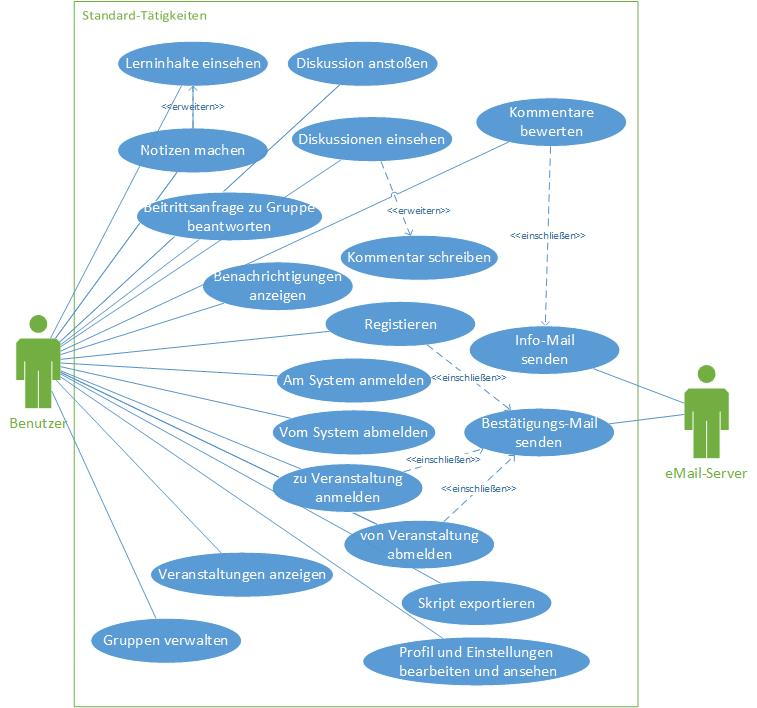
\includegraphics[width=\textwidth]{Bilder/Anwendungsfalldiagramme/Benutzer.jpg}
	\caption{Dies sind alle Aktionen die von einem Benutzer getätigt werden können.}
	\label{AwfBenutzer}
\end{figure}

\begin{figure}[H]
	\centering
	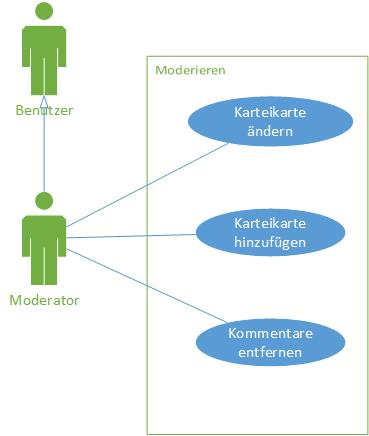
\includegraphics[width=\textwidth]{Bilder/Anwendungsfalldiagramme/Moderator.jpg}
	\caption{Der Moderator erbt alle Anwendungsfälle vom Benutzer. Er kann zusätzlich die Karteikarten und Diskussionen verwalten.}
	\label{AwfModerator}
\end{figure}

\begin{figure}[H]
	\centering
	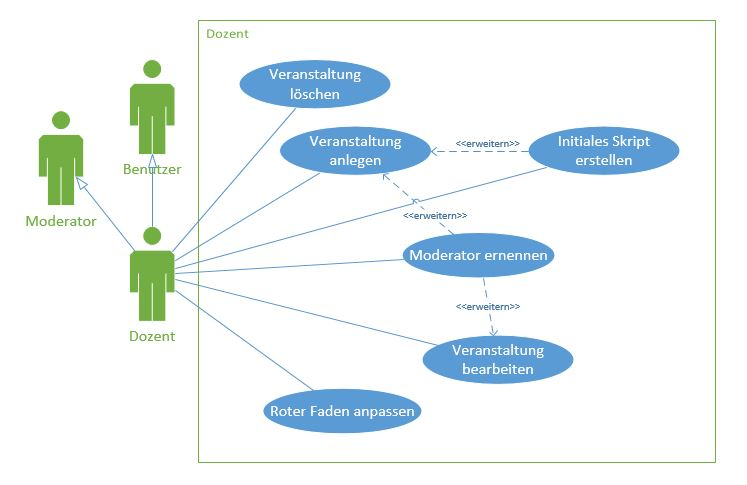
\includegraphics[width=\textwidth]{Bilder/Anwendungsfalldiagramme/abbildung3.jpg}
	\caption{Der Dozent erbt alle Anwendungsfälle vom Benutzer und vom Moderator. Zusätzlich kann er Veranstaltungen verwalten.}
	\label{AwfDozent}
\end{figure}

\begin{figure}[H]
	\centering
	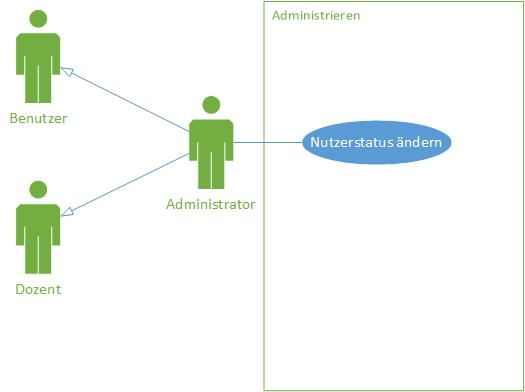
\includegraphics[width=\textwidth]{Bilder/Anwendungsfalldiagramme/Admin.jpg}
	\caption{Der Administrator erbt von allen Akteuren und hat somit alle Rechte. Er kann Nutzer in den Dozenten-Status erheben.}
	\label{AwfAdmin}
\end{figure}

\newpage

\subsubsection{Szenarien}
Alle Anwendungsfälle werden durch Sequenzdiagramme beschrieben. Diese Diagramme beschreiben einen beispielhaften Ablauf und die möglichen Alternativen einer Aktion auf.

\begin{figure}[H]
	\centering
	\paragraph{Registrierung}
	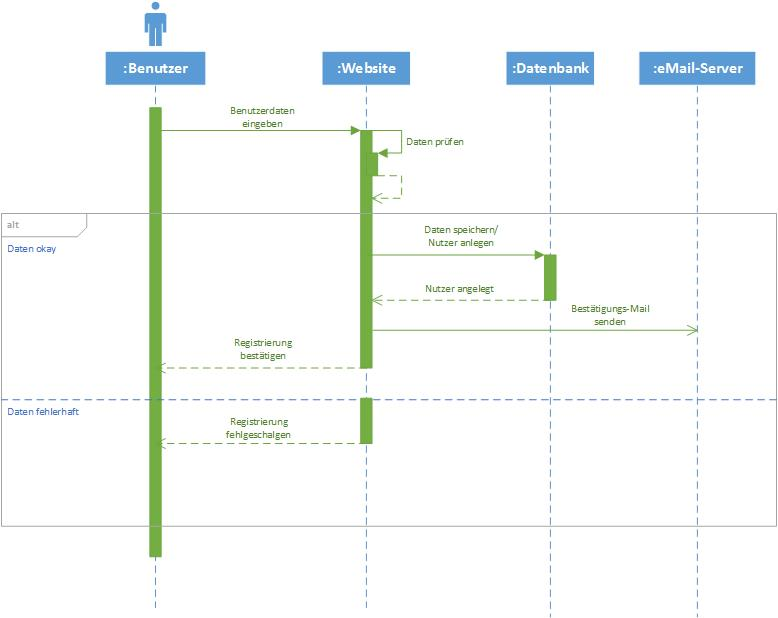
\includegraphics[width=\textwidth]{Bilder/Sequenzdiagramme/Registrierung1.jpg}
	\caption{Die initiale Benutzerregistrierung im System.}
	\label{SzRegistrieren}
\end{figure}
\begin{figure}[H]
	\centering
	\paragraph{Profil bearbeiten}
	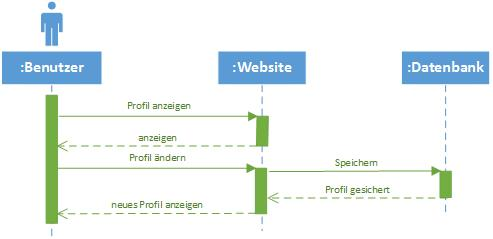
\includegraphics[width=\textwidth]{Bilder/Sequenzdiagramme/ProfilBearbeiten1.jpg}
	\caption{Der Benutzer bearbeitet sein persönliches Profil.}
	\label{SzProfilBearbeiten}
\end{figure}
\begin{figure}[H]
	\centering
	\paragraph{Am System anmelden}
	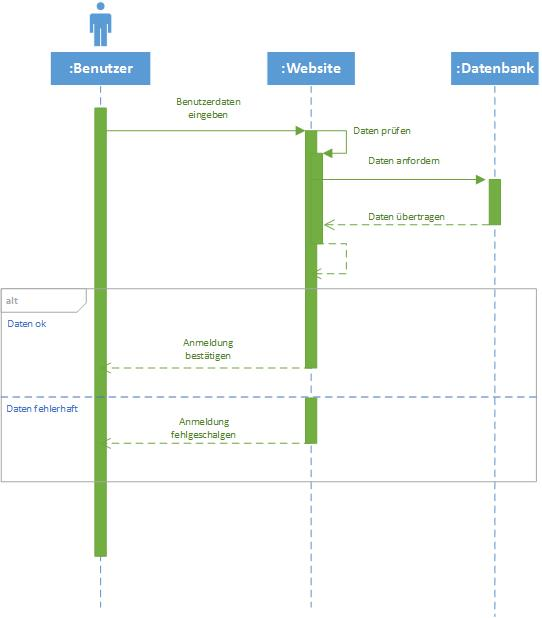
\includegraphics[width=\textwidth]{Bilder/Sequenzdiagramme/AmSystemAnmelden1.jpg}
	\caption{Die Benutzeranmeldung am System.}
	\label{SzAmSystemAnmelden}
\end{figure}
\begin{figure}[H]
	\centering
	\paragraph{Vom System abmelden}
	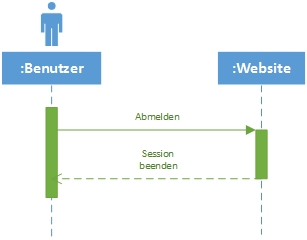
\includegraphics[width=\textwidth]{Bilder/Sequenzdiagramme/VomSystemAbmelden.jpg}
	\caption{Die Benutzerabmeldung}
	\label{SzVomSystemAbmelden}
\end{figure}
\begin{figure}[H]
	\centering
	\paragraph{Zu einer Veranstaltung anmelden}
	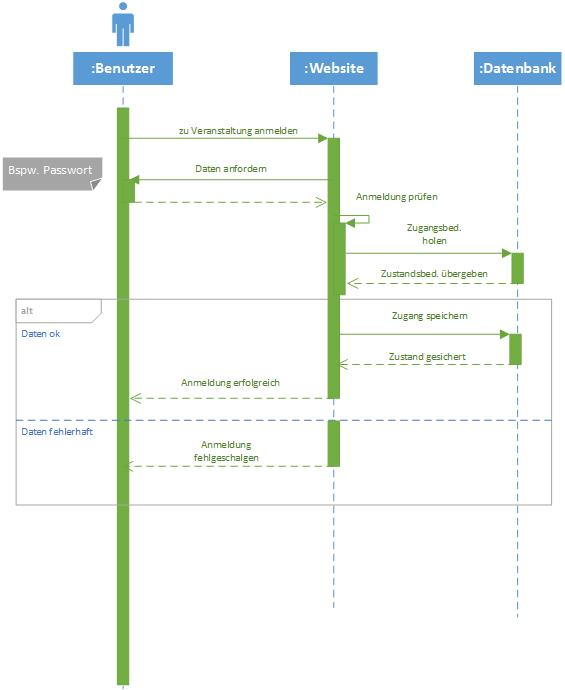
\includegraphics[width=\textwidth]{Bilder/Sequenzdiagramme/ZuVeranstaltungAnmelden1.jpg}
	\caption{Die Anmeldung von einem Benutzer zu einer Veranstaltung.}
	\label{SzZuVeranstaltungAnmelden}
\end{figure}
\begin{figure}[H]
	\centering
	\paragraph{Von einer Veranstaltung abmelden}
	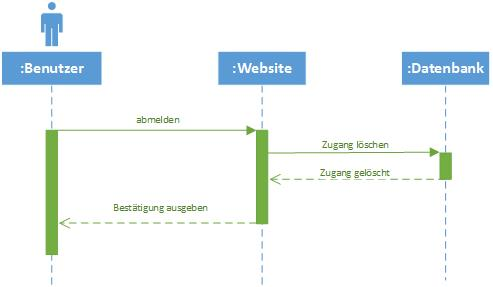
\includegraphics[width=\textwidth]{Bilder/Sequenzdiagramme/VonVeranstaltungAbmelden1.jpg}
	\caption{Der Benutzer meldet sich von einer Veranstaltung ab.}
	\label{SzVonVeranstaltungAbmelden}
\end{figure}
\begin{figure}[H]
	\centering
	\paragraph{Veranstaltung anzeigen}
	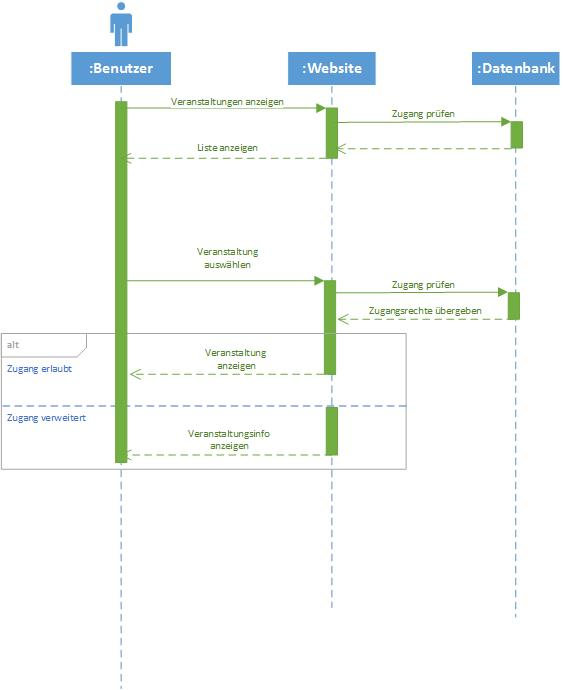
\includegraphics[width=\textwidth]{Bilder/Sequenzdiagramme/VeranstaltungenAnzeigen1.jpg}
	\caption{Der Benutzer zeigt sich alle bestehenden Veranstaltungen an.}
	\label{SzVeranstaltungenAnzeigen}
\end{figure}
\begin{figure}[H]
	\centering
	\paragraph{Eine neue Veranstaltung anlegen}
	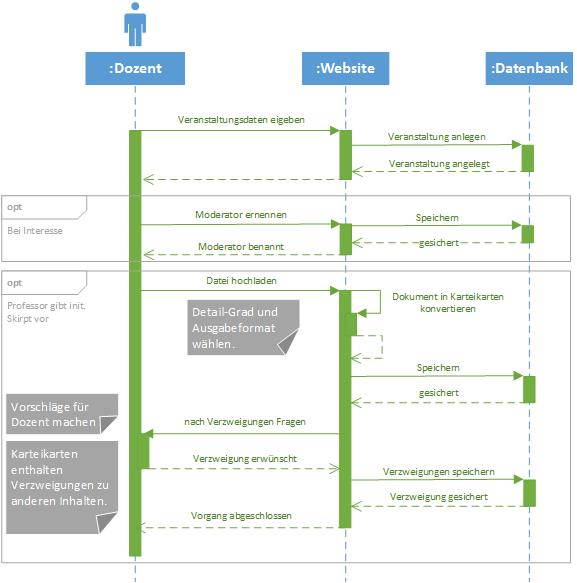
\includegraphics[width=\textwidth]{Bilder/Sequenzdiagramme/VeranstaltungAnlegen1.jpg}
	\caption{Der Dozent erstellt eine neue Veranstaltung.}
	\label{SzVeranstaltungAnlegen}
\end{figure}
\begin{figure}[H]
	\centering
	\paragraph{Eine vorhandene Veranstaltung löschen}
	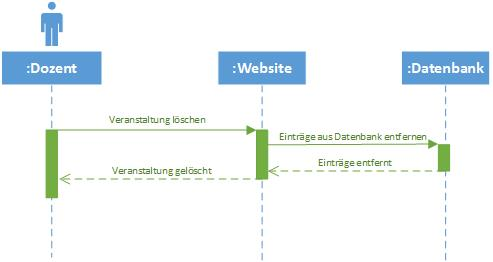
\includegraphics[width=\textwidth]{Bilder/Sequenzdiagramme/VeranstaltungLoeschen1.jpg}
	\caption{Die vom dem Dozenten erstellte Veranstaltungen löschen.}
	\label{SzVeranstaltungLoeschen}
\end{figure}
\begin{figure}[H]
	\centering
	\paragraph{Veranstaltung bearbeiten}
	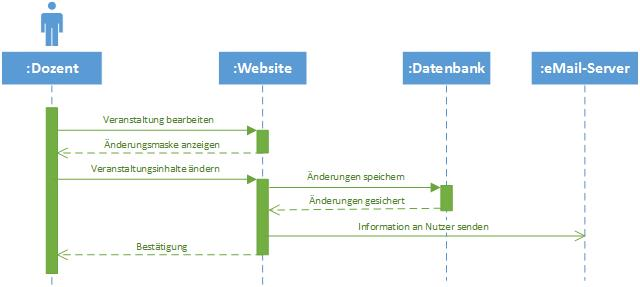
\includegraphics[width=\textwidth]{Bilder/Sequenzdiagramme/VeranstaltungBearbeiten1.jpg}
	\caption{Der Dozent nimmt Änderungen an seiner Veranstaltungen vor.}
	\label{SzVeranstaltungBearbeiten}
\end{figure}
\begin{figure}[H]
	\centering
	\paragraph{Lerninhalt einsehen}
	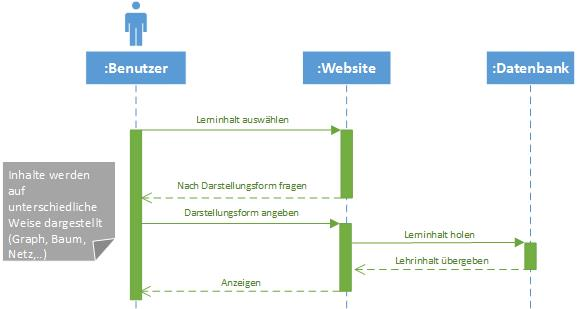
\includegraphics[width=\textwidth]{Bilder/Sequenzdiagramme/LerninhalteEinsehen1.jpg}
	\caption{Der Benutzer zeigt sich eine Diskussion zu einer Karteikarte an.}
	\label{SzLerninhaltEinsehen}
\end{figure}
\begin{figure}[H]
	\centering
	\paragraph{Roter Faden bearbeiten}
	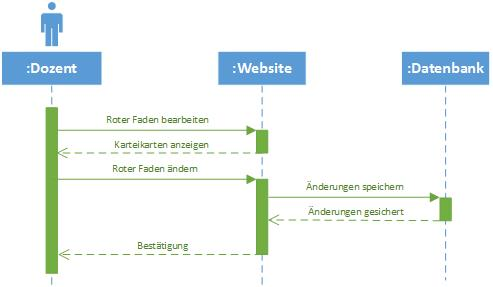
\includegraphics[width=\textwidth]{Bilder/Sequenzdiagramme/RoterFadenBearbeiten1.jpg}
	\caption{Der Dozent nimmt Änderungen am roten Faden vor.}
	\label{SzRoterFaden}
\end{figure}
\begin{figure}[H]
	\centering
	\paragraph{Notizen machen}
	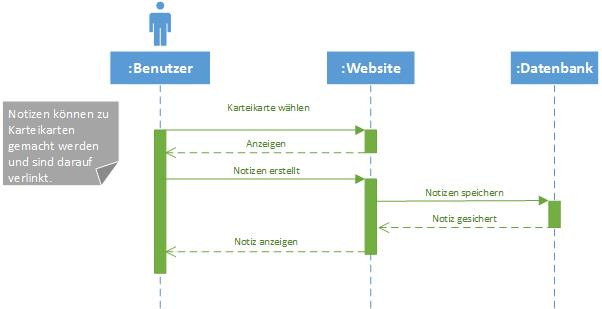
\includegraphics[width=\textwidth]{Bilder/Sequenzdiagramme/NotizenMachen1.jpg}
	\caption{Der Benutzer legt eine Notiz zu einer Karteikarte an.}
	\label{SzNotizenMachen}
\end{figure}
\begin{figure}[H]
	\centering
	\paragraph{Skript exportieren}
	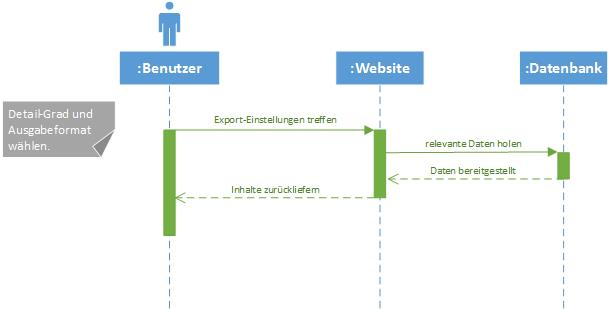
\includegraphics[width=\textwidth]{Bilder/Sequenzdiagramme/SkriptExportieren1.jpg}
	\caption{Der Benutzer exportiert das Skript.}
	\label{SzSkriptExportieren}
\end{figure}
\begin{figure}[H]
	\centering
	\paragraph{Diskussion beginnen}
	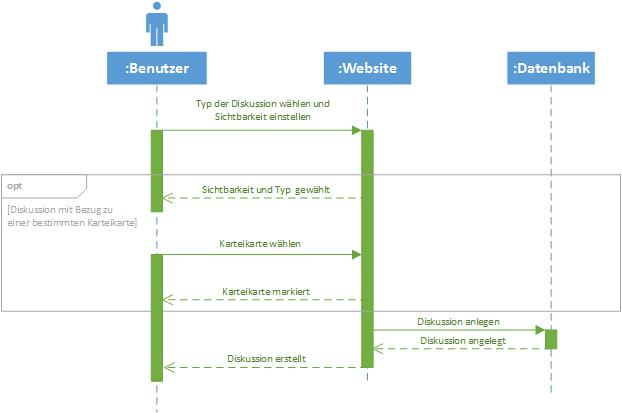
\includegraphics[width=\textwidth]{Bilder/Sequenzdiagramme/DiskussionAnstossen1.jpg}
	\caption{Der Benutzer stößt eine Diskussion zu einer Karteikarte an.}
	\label{SzDiskussionAnstossen}
\end{figure}
\begin{figure}[H]
	\centering
	\paragraph{Diskussion einsehen}
	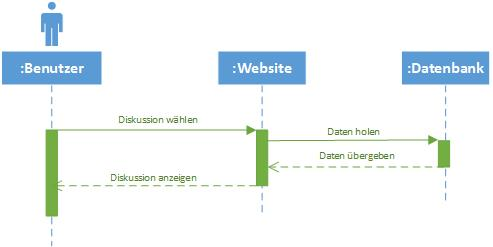
\includegraphics[width=\textwidth]{Bilder/Sequenzdiagramme/DiskussionEinsehen1.jpg}
	\caption{Der Benutzer lässt sich eine Diskussion zu einer Karteikarte anzeigen.}
	\label{SzDiskussionEinsehen}
\end{figure}
\begin{figure}[H]
	\centering
	\paragraph{Kommentar schreiben}
	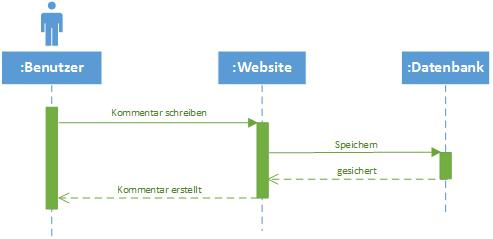
\includegraphics[width=\textwidth]{Bilder/Sequenzdiagramme/KommentarSchreiben1.jpg}
	\caption{Der Nutzer hinterlässt einen Kommentar zu einer Diskussion.}
	\label{SzKommentarSchreiben}
\end{figure}
\begin{figure}[H]
	\centering
	\paragraph{Kommentare bewerten}
	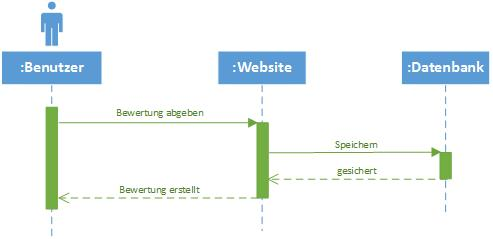
\includegraphics[width=\textwidth]{Bilder/Sequenzdiagramme/KommentareBewerten1.jpg}
	\caption{Der Nutzer bewertet einen Kommentar in einer Diskussion.}
	\label{SzKommentareBewerten}
\end{figure}
\begin{figure}[H]
	\centering
	\paragraph{Kommentare löschen}
	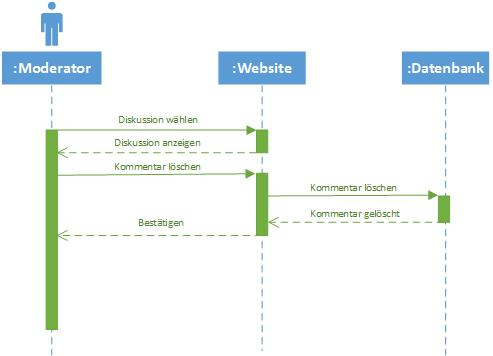
\includegraphics[width=\textwidth]{Bilder/Sequenzdiagramme/KommentareLoeschen1.jpg}
	\caption{Der Moderator löscht nicht relevante Kommentare.}
	\label{SzKommentarLoeschen}
\end{figure}
\begin{figure}[H]
	\centering
	\paragraph{Karteikarte hinzufügen}
	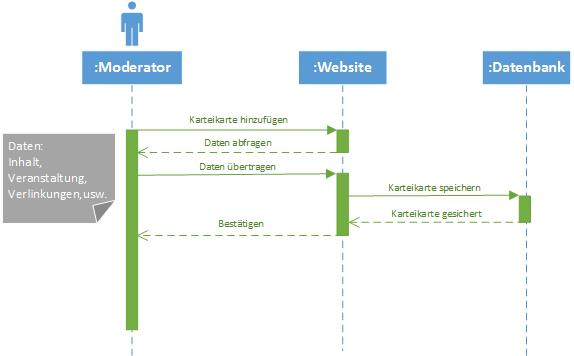
\includegraphics[width=\textwidth]{Bilder/Sequenzdiagramme/KarteikarteHinzufuegen1.jpg}
	\caption{Der Moderator fügt eine neue Karteikarte hinzu.}
	\label{SzKarteikarteHinzufuegen}
\end{figure}
\begin{figure}[H]
	\centering
	\paragraph{Karteikarte ändern}
	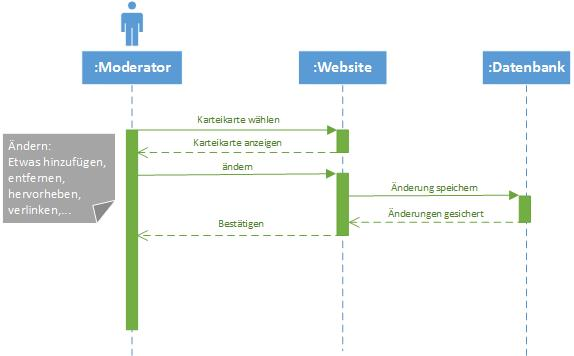
\includegraphics[width=\textwidth]{Bilder/Sequenzdiagramme/KarteikarteAendern1.jpg}
	\caption{Der Moderator ändert eine Karteikarte.}
	\label{SzKarteikarteAendern}
\end{figure}
\begin{figure}[H]
	\centering
	\paragraph{Karteikarte löschen}
	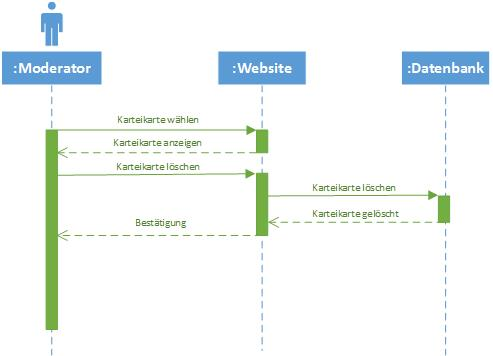
\includegraphics[width=\textwidth]{Bilder/Sequenzdiagramme/KarteikarteLoeschen1.jpg}
	\caption{Der Moderator löscht eine Karteikarte.}
	\label{SzKarteikarteLoeschen}
\end{figure}
\begin{figure}[H]
	\centering
	\paragraph{Gruppe verwalten}
	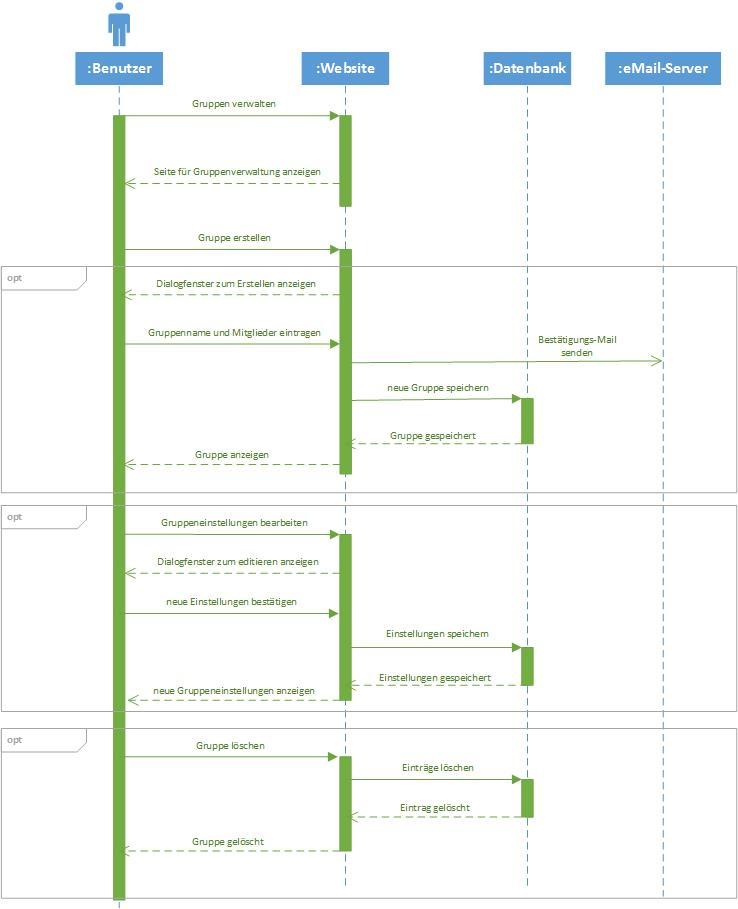
\includegraphics[width=\textwidth]{Bilder/Sequenzdiagramme/GruppenVerwalten1.jpg}
	\caption{Der Benutzer verwaltet die Gruppen.}
	\label{SzGruppenVerwalten}
\end{figure}
\begin{figure}[H]
	\centering
	\paragraph{Beitrittsanfrage zu Gruppe beantworten}
	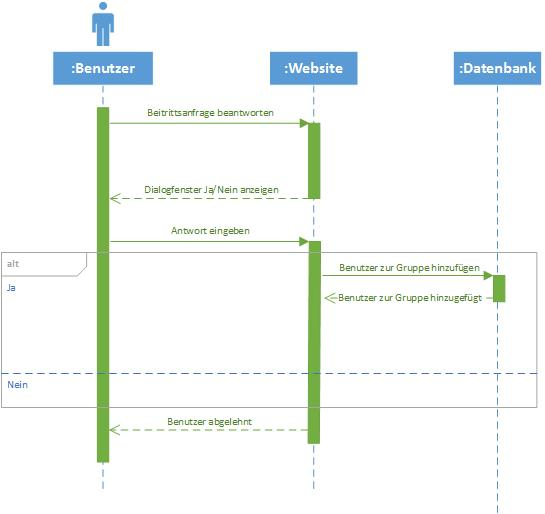
\includegraphics[width=\textwidth]{Bilder/Sequenzdiagramme/BeitrittsanfrageZuGruppe1.jpg}
	\caption{Der Benutzer beantwortet Beitrittsanfragen zu Gruppen.}
	\label{SzBeitrittsanfrageZuGruppe}
\end{figure}
\begin{figure}[H]
	\centering
	\paragraph{Benachrichtigungen anzeigen}
	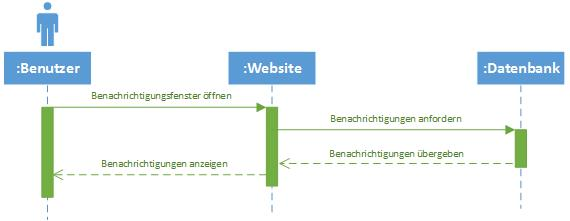
\includegraphics[width=\textwidth]{Bilder/Sequenzdiagramme/BenachrichtigungenAnzeigen1.jpg}
	\caption{Der Benutzer zeigt sich seine Benachrichtigungen an.}
	\label{SzBenachrichtigungen}
\end{figure}
\begin{figure}[H]
	\centering
	\paragraph{Nutzerstatus ändern}
	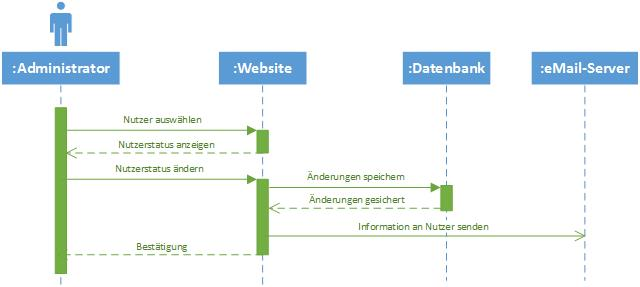
\includegraphics[width=\textwidth]{Bilder/Sequenzdiagramme/NutzerstatusAendern1.jpg}
	\caption{Der Administrator ändert die Profildaten eines Benutzers.}
	\label{SzNutzerstatusAendern}
\end{figure}

\begin{figure}[H]
	\centering
	\paragraph{Mail versenden}
	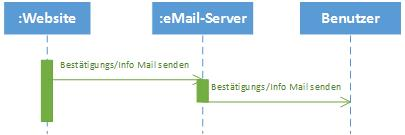
\includegraphics[width=\textwidth]{Bilder/Sequenzdiagramme/MailVersenden1.jpg}
	\caption{Das System sendet eine Mail an den Benutzer.}
	\label{SzMailVersenden}
\end{figure}


\subsubsection{Systemaufgabe}
Hier werden alle Systemaufgaben, die dazugehörigen Teilnehmer und jeweils eine kurze Beschreibung aufgelistet. Außerdem wird jede Anforderung mit einer Markierung (von nicht sehr von Bedeutung [-2]  bis [2] sehr wichtig) versehen, die darlegt, wie wichtig diese Anforderung ist.

\paragraph{Funktionale Anforderungen}
\subparagraph{Benutzer - Anwendungsfall "Registrieren" (2)}\mbox{}\\
\textbf{Eingabe der Daten}\\
\begin{tabular}{l| p{10cm}}
\hline 
Beteiligt & Anonym, System \\ 
Beschreibung & Eine anonyme Person kann ihre Zugangsdaten bei der Registrierung eingeben. Mit diesen Daten wird dann ein neuer Benutzer im System angemeldet.\\ 
\end{tabular}\\

\textbf{Registrierung bestätigen}\\
\begin{tabular}{l|p{10cm}}
\hline 
Beteiligt    & Benutzer, System, eMail-Server \\ 
Beschreibung & Die erfolgreiche Anmeldung wird dem Benutzer  \\
 			 & per Dialog und zusätzlich per Mail bestätigt. \\ 
\end{tabular} 

\newpage
\subparagraph{Benutzer - Anwendungsfall \glqq Am System anmelden \grqq (2)}\mbox{}

\textbf{Eingabe der Zugangsdaten}\\
\begin{tabular}{l|p{10cm}}
\hline 
Beteiligt & Benutzer, System \\ 
Beschreibung & Der Nutzer gibt seine Zugangsdaten ein. Wenn die Anmeldung erfolgreich war wird der Nutzer am System angemeldet. Bei inrorrekten Zugangsdaten erscheint eine Fehlermeldung. \\ 
\end{tabular}\\


\textbf{Anmeldung bestätigen}\\
\begin{tabular}{l|p{10cm}}
\hline 
Beteiligt & Benutzer, System \\ 
Beschreibung & Das System bestätigt dem Nutzer die Anmeldung. \\ 
\end{tabular}\\\\


\subparagraph{Benutzer - Anwendungsfall \glqq Vom System abmelden \grqq (2)}\mbox{}

\textbf{Abmelden}\\
\begin{tabular}{l|p{10cm}}
\hline 
Beteiligt & Benutzer, System \\ 
Beschreibung & Bei der Abmeldung vom System wird die Session vom Benutzer beendet.\\ 
\end{tabular}\\

\textbf{Abmeldung bestätigen}\\
\begin{tabular}{l|p{10cm}}
\hline 
Beteiligt & Benutzer, System \\ 
Beschreibung &  Das System zeigt an, dass das Abmelden erfolgreich war. \\ 
\end{tabular}\\\\



\subparagraph{Benutzer - Anwendungsfall \glqq Veranstaltungen anzeigen \grqq (2)}\mbox{}

\textbf{Alle Veranstaltungen anzeigen}\\
\begin{tabular}{l|p{10cm}}
\hline 
Beteiligt & Benutzer, System  \\ 
Beschreibung & Das System zeigt dem Benutzer alle verfügbaren Veranstaltungen an. \\ 
\end{tabular}\\ 

\textbf{Veranstaltungen auswählen und anzeigen}\\
\begin{tabular}{l|p{10cm}}
\hline 
Beteiligt & Benutzer, System \\ 
Beschreibung & Das System zeigt dem Benutzer alle Veranstaltung an, an denen er nicht angemeldet ist. Ist der Benutzer schon zu einer Veranstaltung angemeldet, wird ihm direkt die eigentliche Veranstaltungsseite angezeigt. \\ 
\end{tabular} \\\\

\newpage

\subparagraph{Benutzer - Anwendungsfall \glqq Zu Veranstaltung anmelden \grqq (2)}\mbox{}

\textbf{Zu Veranstaltung anmelden}\\
\begin{tabular}{l|p{10cm}}
\hline 
Beteiligt & Benutzer, System \\ 
Beschreibung & Nachdem der Benutzer die Zugangsdaten zur Veranstaltung korrekt angegeben hat, wird die Zugangsberechtigung vom System übernommen und der Benutzer wird zur Veranstaltungsseite weitergeleitet. Andernfalls wird ihm eine Fehlermeldung angezeigt.\\ 
\end{tabular}\\\\


\subparagraph{Benutzer - Anwendungsfall \glqq Von Veranstaltung abmelden\grqq (0)}\mbox{}

\textbf{Von Veranstaltung abmelden}\\
\begin{tabular}{l|p{10cm}}
\hline 
Beteiligt & Benutzer, System \\ 
Beschreibung & Das System meldet den Benutzer vom System ab und zeigt Ihm an ob der Vorgang erfolgreich war. \\ 
\end{tabular}\\\\


\subparagraph{Benutzer - Anwendungsfall \glqq Skript exportieren\grqq (-1)}\mbox{}

\textbf{Exportseite anzeigen und Skript wählen}\\
\begin{tabular}{l|p{10cm}}
\hline 
Beteiligt & Benutzer, System \\ 
Beschreibung & Der Nutzer bekommt eine Exportoberfläche angezeigt, auf der er den zu exportierenden Lernstoff wählen kann. \\ 
\end{tabular}\\

\textbf{Exporteinstellungen treffen}\\
\begin{tabular}{l|p{10cm}}
\hline 
Beteiligt & Benutzer, System \\ 
Beschreibung & Der Benutzer hat die Möglichkeit die Export-Einstellungen festzulegen. \\ 
\end{tabular}\\

\textbf{Skript exportieren}\\
\begin{tabular}{l|p{10cm}}
\hline 
Beteiligt & Benutzer, System \\ 
Beschreibung & Das System generiert das Dokument und bietet es dem Nutzer zum Download an. \\ 
\end{tabular}\\\\


\subparagraph{Benutzer - Anwendungsfall \glqq Profil und Einstellungen bearbeiten und ansehen\grqq  (2)}\mbox{}

\textbf{Profil anzeigen}\\
\begin{tabular}{l|p{10cm}}
\hline 
Beteiligt & Benutzer, System \\ 
Beschreibung & Der Nutzer kann sein eigenes Profil oder das anderer Benutzer einsehen. \\ 
\end{tabular}\\

\textbf{Profil bearbeiten}\\
\begin{tabular}{l|p{10cm}}
\hline 
Beteiligt & Benutzer, System \\ 
Beschreibung & Jeder Nutzer kann sein eigenes Profil bearbeiten. \\ 
\end{tabular}\\ 

\textbf{Einstellungen bearbeiten}\\
\begin{tabular}{l|p{10cm}}
\hline 
Beteiligt & Benutzer, System \\ 
Beschreibung & Das System bietet dem Nutzer eine Oberfläche um sämtliche Einstellungen festzulegen. \\ 
\end{tabular}\\

\textbf{Einstellungen- und Profil-Änderungen speichern}\\
\begin{tabular}{l|p{10cm}}
\hline 
Beteiligt &  Benutzer, System \\ 
Beschreibung & Das System bestätigt dem Benutzer die erfolgreiche Änderung oder gibt eine Fehlermeldung aus. \\ 
\end{tabular}\\\


\subparagraph{Benutzer - Anwendungsfall \glqq Diskussion anstoßen\grqq (1)}\mbox{}

\textbf{Neue Diskussion erstellen}\\
\begin{tabular}{l|p{10cm}}
\hline 
Beteiligt & Benutzer, System \\ 
Beschreibung & Jeder Nutzer kann eine neue Diskussion zu einer Karteikarte erstellen. \\ 
\end{tabular}\\

\textbf{Sichtbarkeit einstellen}\\
\begin{tabular}{l|p{10cm}}
\hline 
Beteiligt & Benutzer, System \\ 
Beschreibung & Der Nutzer kann beim Erstellen die Sichtbarkeit der Diskussion einstellen (Öffentlich ersichtlich, nur in der Veranstaltung, nur in der Gruppe). \\ 
\end{tabular}\\\\


\subparagraph{Benutzer - Anwendungsfall \glqq Kommentare machen\grqq (1)}\mbox{}

\textbf{Kommentar hinzufügen}\\
\begin{tabular}{l|p{10cm}}
\hline 
Beteiligt & Benutzer, System \\ 
Beschreibung & Jeder Benutzer muss, wenn er die notwendigen Rechte besitzt, Kommentare zu einer Diskussion hinzufügen. \\ 
\end{tabular}\\\\ 


\subparagraph{Benutzer - Anwendungsfall \glqq Notizen machen\grqq (1)}\mbox{}

\textbf{Notizen hinzufügen}\\
\begin{tabular}{l|p{10cm}}
\hline 
Beteiligt & Benutzer, System \\ 
Beschreibung & Jeder Benutzer muss sich zu einer Karteikarte Notizen machen. \\ 
\end{tabular}\\\\


\subparagraph{Benutzer - Anwendungsfall \glqq Kommentare bewerten\grqq (-1)}\mbox{}

\textbf{Kommentar bewerten}\\
\begin{tabular}{l|p{10cm}}
\hline 
Beteiligt & Benutzer, Moderator, System \\ 
Beschreibung & Jeder Benutzer kann, wenn er die notwendigen Rechte(Sichtbarkeit) hat, bewerten. Ein Moderator kann alle Kommentare  bewerten egal welche Sichtbarkeit dieser besitzt. \\ 
\end{tabular}\\\\


\subparagraph{Benutzer - Anwendungsfall \glqq Gruppen verwalten\grqq (-2)}\mbox{}

\textbf{Gruppe erstellen}\\
\begin{tabular}{l|p{10cm}}
\hline 
Beteiligt & Benutzer, System \\ 
Beschreibung & Jeder Benutzer besitzt Zugriff auf eine Gruppenerstellungsmaske, um eine neue Gruppe hinzufügen. \\ 
\end{tabular}\\

\textbf{Gruppe löschen}\\
\begin{tabular}{l|p{10cm}}
\hline 
Beteiligt & Benutzer, System \\ 
Beschreibung & Jeder Benutzer besitzt Zugriff auf ein Menü, um seine selbst erstellten Gruppen zu löschen. \\ 
\end{tabular}\\

\textbf{Gruppe editieren}\\
\begin{tabular}{l|p{10cm}}
\hline 
Beteiligt & Benutzer, System \\ 
Beschreibung & Jeder Benutzer hat die Möglichkeit, seine selbst erstellten Gruppen zu editieren, indem er bspw. neue Mitglieder hinzufügt. \\ 
\end{tabular}\\\\


\subparagraph{Benutzer - Anwendungsfall \glqq Benachrichtigungen anzeigen\grqq  (1)}\mbox{}

\textbf{Benachrichtigungen anzeigen}\\
\begin{tabular}{l|p{10cm}}
\hline 
Beteiligt & Benutzer, System \\ 
Beschreibung & Jedem Benutzer werden immer aktuelle Informationen wie eine Beitrittsanfrage zu einer Gruppe, oder neue Kommentare angezeigt. \\ 
\end{tabular}\\\\
 


\subparagraph{Benutzer - Anwendungsfall \glqq Lerninhalte anzeigen\grqq  (2)}\mbox{}

\textbf{Lerninhalte anzeigen}\\
\begin{tabular}{l|p{10cm}}
\hline 
Beteiligt & Benutzer, System  \\ 
Beschreibung & Jedem Benutzer werden die Lerninhalte zu einer Veranstaltung angezeigt, zu der er angemeldet ist. \\ 
\end{tabular}\\


\subparagraph{Benutzer - Anwendungsfall \glqq Beitrittsanfrage zu Gruppe beantworten\grqq (-2)}\mbox{}

{\textbf{Beitrittsanfragen beantworten}\\
\begin{tabular}{l|p{10cm}}
\hline 
Beteiligt & Benutzer, Moderator, System \\ 
Beschreibung & Jeder Benutzer kann über eine Oberfläche ausstehende Beitrittsanfragen annehmen oder ablehnen. \\ 
\end{tabular}\\\\


\subparagraph{Dozent - Anwendungsfall \glqq Veranstaltung anlegen\grqq (2)}\mbox{}

\textbf{Veranstaltungsdaten eingeben}\\
\begin{tabular}{l|p{10cm}}
\hline 
Beteiligt & Dozent, System \\ 
Beschreibung & Es gibt eine Oberfläche, wo der Dozent die Veranstaltungsdaten(Name, Beschreibung, Zugangspasswort,..) eingeben kann. Daraufhin wird eine neue Veranstaltung im System angelegt. Siehe auch Anwendungsfall \glqq Initiales Skript importieren \grqq . \\ 
\end{tabular} \\\\


\subparagraph{Dozent - Anwendungsfall \glqq Moderator ernennen\grqq (2)}\mbox{}

\textbf{Moderator ernennen}\\
\begin{tabular}{l|p{10cm}}
\hline 
Beteiligt & Dozent, System \\ 
Beschreibung & Der Dozent kann für seine Veranstaltungen Moderatoren angeben. \\ 
\end{tabular}\\\\


\subparagraph{Dozent - Anwendungsfall \glqq Initiales Skript erstellen\grqq (1)}\mbox{}

\textbf{Importseite anzeigen und Skript hochladen}\\
\begin{tabular}{l|p{10cm}}
\hline 
Beteiligt & Dozent, System \\ 
Beschreibung & Der Dozent bekommt eine Importoberfläche angezeigt und lädt ein Skript hoch. Nachdem der Dozent die Import-Einstellungen angegeben hat, konvertiert das System dieses Skript in die Karteikarten-Repräsentation, erstellt den initialen roten Faden und bietet die Möglichkeit zusätzliche Verlinkungen einzufügen. \\ 
\end{tabular}\\\\

\newpage

\subparagraph{Dozent - Anwendungsfall \glqq Veranstaltung bearbeiten\grqq (0)}\mbox{}

\textbf{Veranstaltung bearbetien}\\
\begin{tabular}{l|p{10cm}}
\hline 
Beteiligt & Dozent, System \\ 
Beschreibung & Der Dozent kann seine eigenen Veranstaltungen bearbeiten, indem er neue Moderatoren hinzufügt, andere löscht, optionale Features ein oder aus schaltet oder die Veranstaltungsbeschreibung ändert. \\ 
\end{tabular}\\\\


\subparagraph{Dozent - Anwendungsfall \glqq Roter Faden anpassen\grqq (2)}\mbox{}

\textbf{Roter Faden anpassen}\\
\begin{tabular}{l|p{10cm}}
\hline 
Beteiligt & Dozent, System \\ 
Beschreibung & Der Dozent kann den initialen roten Faden anpassen, indem er diesen Menüpunkt einfach bei der entsprechenden Veranstaltung wählt. Dann werden ihm die Karteikarten, die den roten Faden bilden als Liste angezeigt. Jetzt kann er andere Karteikarten einfügen, bestehende entfernen oder umsortieren. \\ 
\end{tabular}\\\\


\subparagraph{Moderator - Anwendungsfall \glqq Karteikarte hinzufügen\grqq (2)}\mbox{}

\textbf{Karteikarte hinzufügen}\\
\begin{tabular}{l|p{10cm}}
\hline 
Beteiligt & Moderator, System \\ 
Beschreibung & Der Moderator kann Karteikarten zum bestehenden Lernstoff hinzufügen. Hierbei muss er das Verweisziel angeben und Attribute setzen. \\ 
\end{tabular}\\\\

\subparagraph{Moderator - Anwendungsfall \glqq Karteikarte ändern\grqq (2)}\mbox{}

\textbf{Karteikarte ändern}\\
\begin{tabular}{l|p{10cm}}
\hline 
Beteiligt & Moderator, System \\ 
Beschreibung & Der Moderator muss Änderungen der Karteikarten vornehmen können. \\ 
\end{tabular}\\\\

\newpage

\subparagraph{Moderator - Anwendungsfall \glqq Karteikarte entfernen\grqq (2)}\mbox{}

\textbf{Karteikarte entfernen}\\
\begin{tabular}{l|p{10cm}}
\hline 
Beteiligt & Moderator, System \\ 
Beschreibung & Der Moderator soll Karteikarten entfernen können. \\ 
\end{tabular}\\\\


\subparagraph{Moderator - Anwendungsfall \glqq Kommentare entfernen\grqq (2)}\mbox{}

\textbf{Karteikarte entfernen}\\
\begin{tabular}{l|p{10cm}}
\hline 
Beteiligt & Moderator, System \\ 
Beschreibung & Der Moderator muss Kommentare entfernen können. \\ 
\end{tabular}\\\\

\subparagraph{Administrator - Anwendungsfall \glqq Nutzerstatus ändern\grqq (2)}\mbox{}

\textbf{Nutzerstatus ändern}\\
\begin{tabular}{l|p{10cm}}
\hline 
Beteiligt & Administrator, System \\ 
Beschreibung & Der Administrator kann Benutzer in den Dozentenstatus erheben. Das heißt, dass sich Dozenten zu Beginn als Studenten im System registrieren müssen. \\ 
\end{tabular}\\\\ 

\paragraph{Nicht funktionale Anforderungen}\mbox{}\\
Hier werden alle nicht funktionalen Anforderungen aufgelistet, denen das System gerecht werden muss. Auch hier wird jeder Abschnitt mit einer Nummer zwischen -2 und 2 versehen. Diese Nummer repräsentiert auch hier, wie wichtig diese Anforderung für das System ist.
\subparagraph{Benutzerfreundlichkeit (2)}
\begin{itemize}
\item Ein noch so gut funktionierendes System ist wertlos, wenn die Handhabung des Systems so schlecht ist, dass sich kein Anwender lange damit auseinandersetzen will. 
\item Es muss intuitiv und einfach zu bedienen sein.
\end{itemize}
\subparagraph{Robustheit (1)}
\begin{itemize}
\item Das System muss robust gegenüber Abstürzen sein. 
\item Es sollten keine unerwarteten Zustände auftreffen. Und falls doch, sollte sich das System so verhalten, dass keine Daten verloren gehen.
\end{itemize}
\subparagraph{Performance (0)}
\begin{itemize}
\item Das System sollte effizient sein.
\item Viele Datenbankzugriffe erfordern eine effiziente Strukturierung der Daten.
\item Es soll auf langsame Web-Plugins verzichtet werden, das diese die Geschwindikeit des Systems nur beeinträchtigen würden. 
\end{itemize}
\subparagraph{Sicherheit (1)}
\begin{itemize}
\item Die Sichtbarkeit und Zugangsrechte sollen einwandfrei funktionieren.
\item Die privaten Daten wie z.b. Notizen sollten nur vom Erzeuger eingesehen werden können.
\item Verbindungen sollten immer verschlüsselt sein.
\end{itemize}
\subparagraph{Verfügbarkeit (1)}
\begin{itemize}
\item Das System soll nicht nur aus dem Uni-Netz sondern auch Weltweit über das Web genutzt werden können.
\item Es sollte zu Wartungszwecken nicht abgeschaltet werden müssen.
\end{itemize}
\subparagraph{Wartbarkeit (-1)}
\begin{itemize}
\item Es soll eine eigene Oberfläche für Administratoren geben. Diese soll  die Wartung des Systems erleichtern.
\end{itemize}
\subparagraph{Darstellungsunabhängigkeit (2)}
\begin{itemize}
\item Die Lehrinhalte müssen unabhängig von der Darstellung gespeichert sein.
\end{itemize}
\subparagraph{Plattformunabhängigkeit (2)}
\begin{itemize}
\item Das System soll als unabhängige Webanwendung implementiert werden.
\end{itemize}

\end{document}
